% MRVA Timing Diagram: Two-Session Execution with Fair Scheduling
% Compile with: lualatex timing-diagram-tikz.tex
%
% A3 landscape, two-page sequence diagram showing state progression
% when two users submit jobs to the MRVA system.

\documentclass[11pt]{article}
\usepackage[a3paper, landscape, margin=1.8cm]{geometry}
\pagestyle{empty}

% Fonts
\usepackage{fontspec}
\setmainfont{Fira Sans}
\setmonofont{IBMPlexMono-Light}
\renewcommand{\familydefault}{\sfdefault}

% TikZ
\usepackage{tikz}
\usetikzlibrary{arrows.meta, calc, backgrounds, fit, decorations.pathreplacing}

% Math (sans serif math via mathastext)
\usepackage{amsmath}
\usepackage{mathastext}

% Colors
\usepackage{xcolor}
\definecolor{u1}{RGB}{31, 119, 180}       % blue -- U_1 / J_1
\definecolor{u2}{RGB}{214, 39, 40}        % red  -- U_2 / J_2
\definecolor{dbcol}{RGB}{44, 160, 44}     % green -- database
\definecolor{mqcol}{RGB}{148, 103, 189}   % purple -- RabbitMQ
\definecolor{schedcol}{RGB}{255, 127, 14} % orange -- scheduler
\definecolor{argocol}{RGB}{127, 127, 127} % gray -- Argo/infra
\definecolor{timecol}{RGB}{80, 80, 80}    % dark gray -- time labels

% -----------------------------------------------------------------------
\begin{document}

\begin{center}
  {\LARGE\bfseries MRVA Timing Diagram: Two-Session Execution}\\[0.3cm]
  {\large Fair Scheduling with Two Workers}\\[0.2cm]
  {\small
    $W{=}2$ (max workers), \quad
    $T_{\text{poll}}{=}10\text{s}$, \quad
    Job duration $= 30\text{s}$, \quad
    Workers: $\alpha_1, \alpha_2$
    \qquad
    \textbf{Legend:}\;
    \tikz[baseline=-0.5ex]{\fill[u1!30,draw=u1](0,0)rectangle(0.5,0.25);}\;U$_1$ jobs\quad
    \tikz[baseline=-0.5ex]{\fill[u2!30,draw=u2](0,0)rectangle(0.5,0.25);}\;U$_2$ jobs\quad
    \tikz[baseline=-0.5ex]{\draw[-{Stealth},semithick](0,0.12)--(0.7,0.12);}\;sync\quad
    \tikz[baseline=-0.5ex]{\draw[-{Stealth},semithick,dashed](0,0.12)--(0.7,0.12);}\;async (MQ)
  }
\end{center}

\vspace{0.3cm}

\noindent\makebox[\textwidth][c]{%
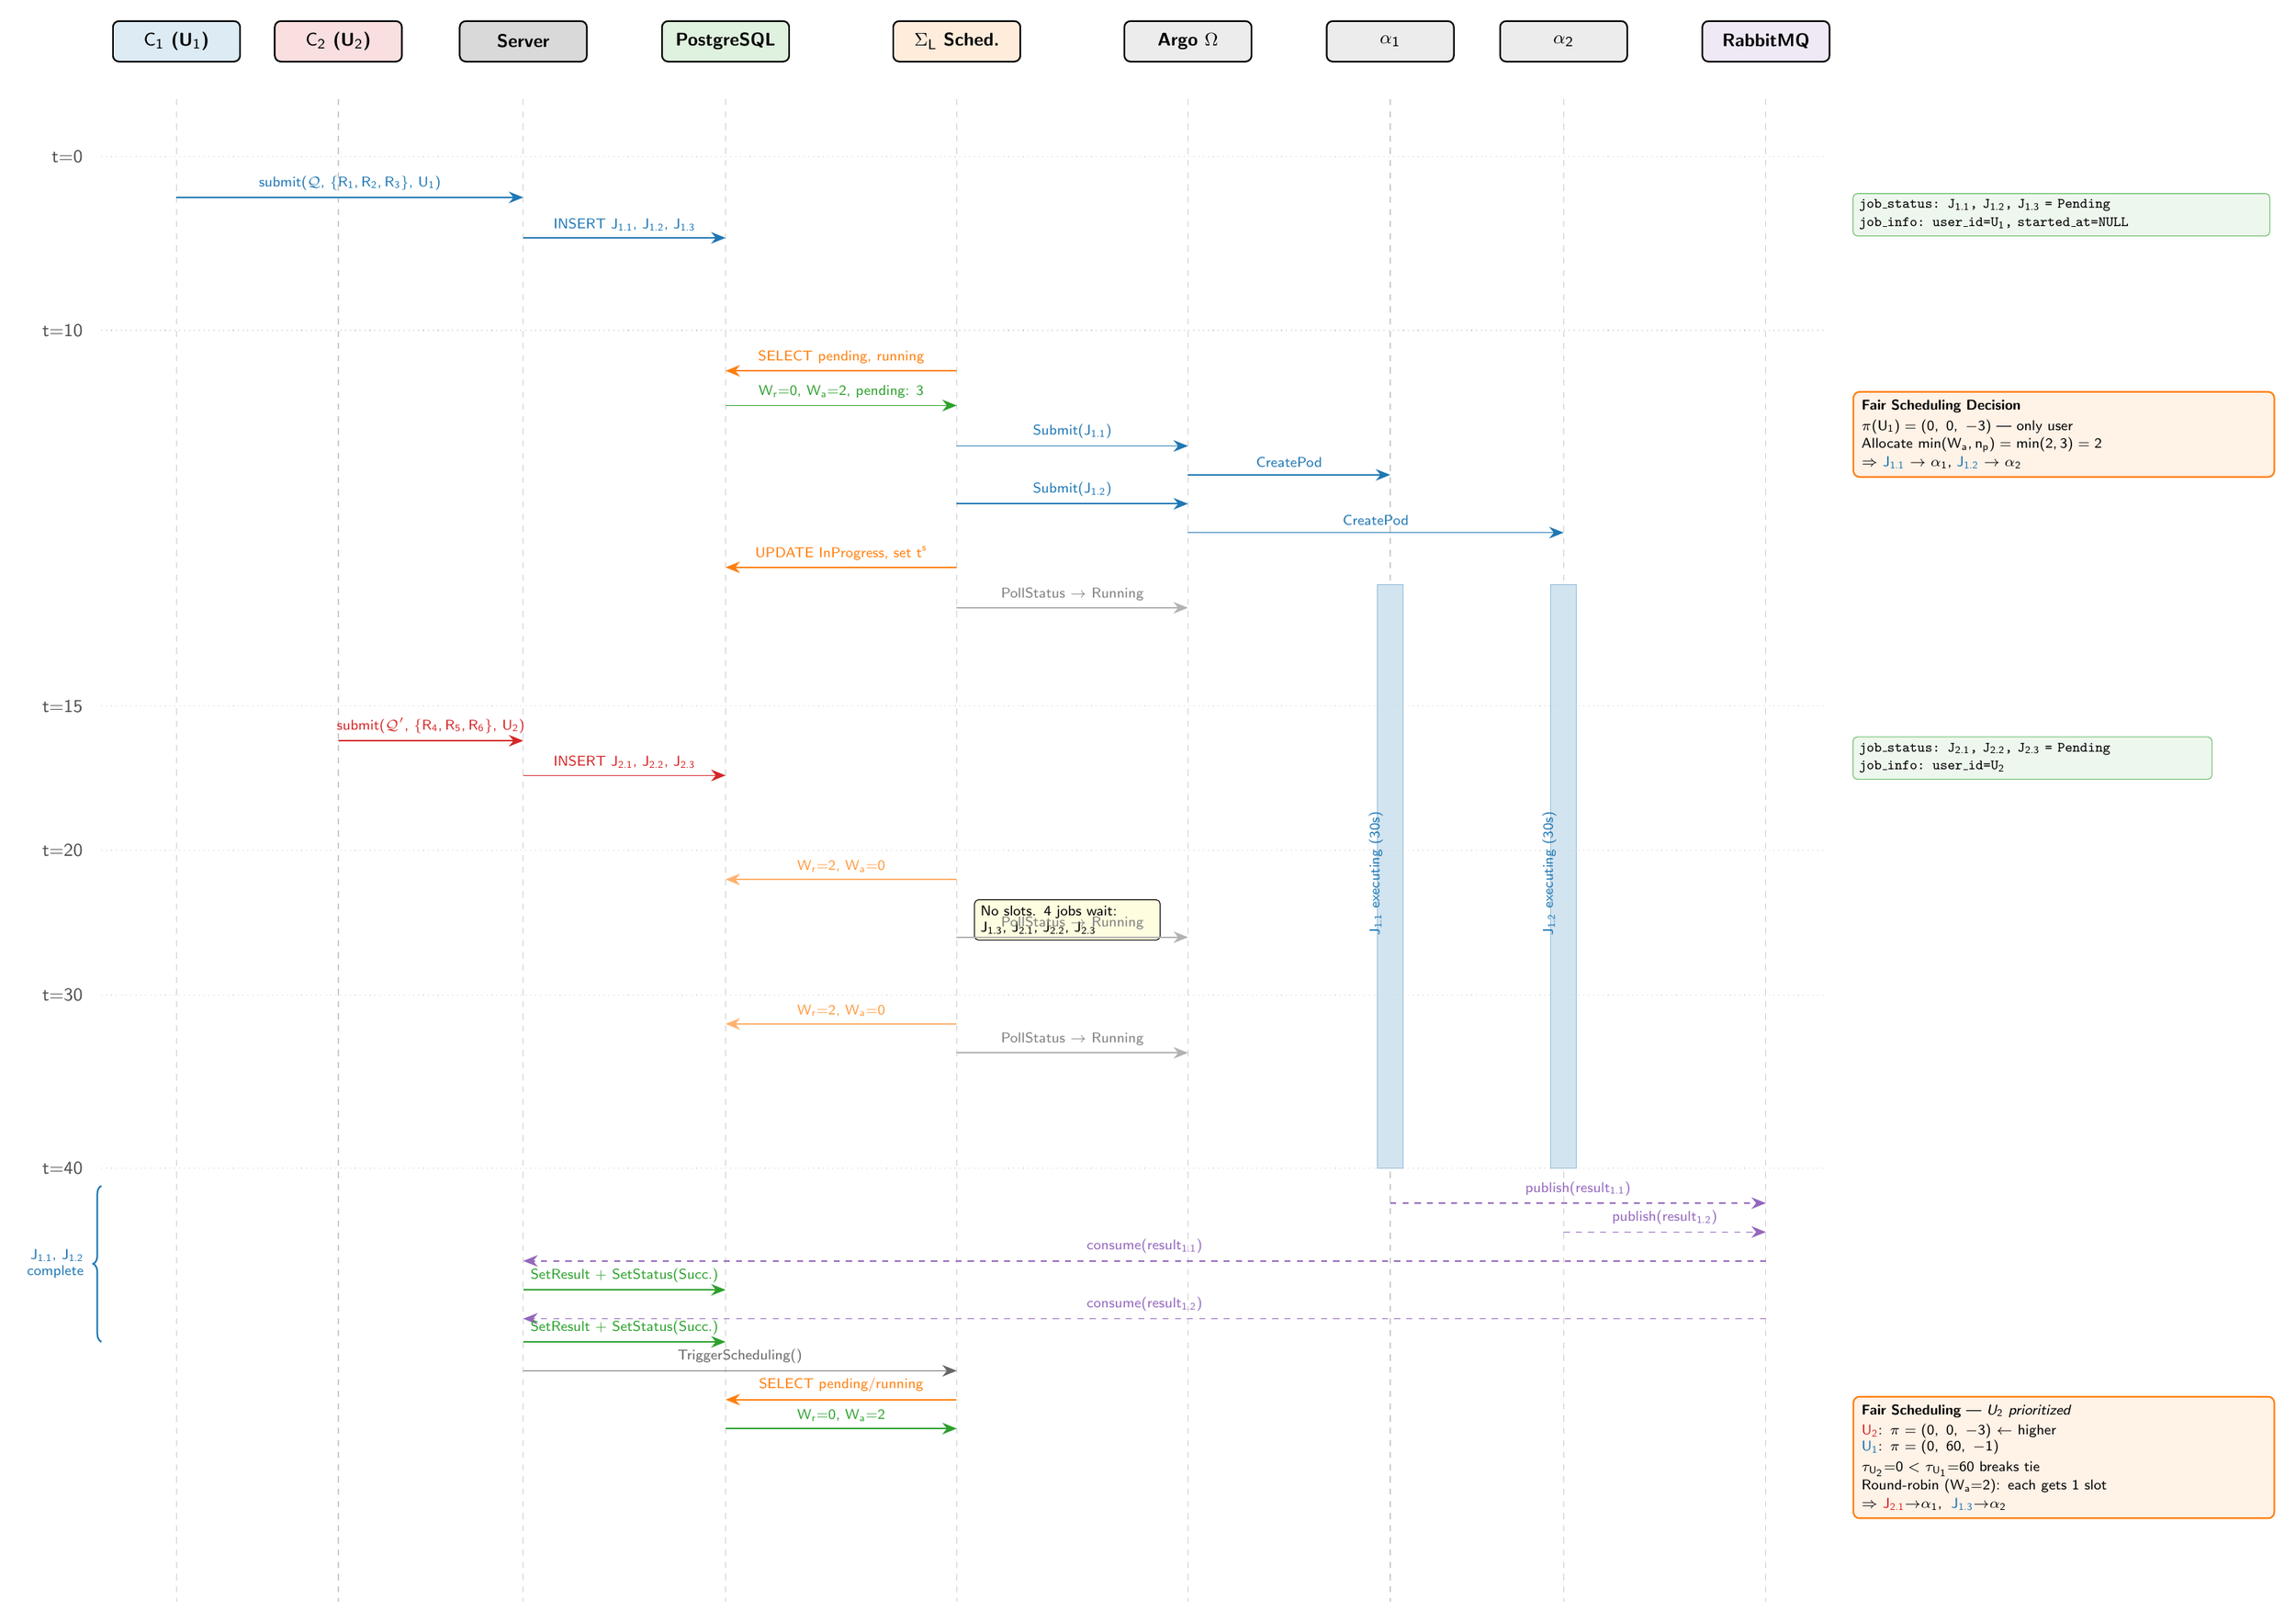
\begin{tikzpicture}[
  x=1cm, y=1cm,
  %
  % Arrow styles
  msg/.style    = {-{Stealth[length=2.5mm, width=2mm]}, semithick, #1},
  msg/.default  = {black},
  amsg/.style   = {-{Stealth[length=2.5mm, width=2mm]}, semithick, dashed, #1},
  amsg/.default = {black},
  %
  % Participant header box
  partbox/.style = {draw, thick, rounded corners=3pt, minimum width=2.2cm,
                    minimum height=0.7cm, font=\small\bfseries, fill=#1!15,
                    text=black},
  %
  % Annotation styles
  note/.style    = {draw, rounded corners=2pt, fill=yellow!12,
                    font=\scriptsize, text width=#1, align=left, inner sep=3pt},
  note/.default  = {3.5cm},
  schedbox/.style = {draw=schedcol, thick, rounded corners=3pt, fill=schedcol!10,
                     font=\scriptsize, text width=#1, align=left, inner sep=4pt},
  schedbox/.default = {5cm},
  dbstate/.style = {draw=dbcol!70, rounded corners=2pt, fill=dbcol!8,
                    font=\scriptsize\ttfamily, text width=#1, align=left, inner sep=3pt},
  dbstate/.default = {5.5cm},
  %
  % Time label
  tmark/.style = {font=\small\bfseries, text=timecol, anchor=east},
]

% ======================================================================
% PARTICIPANT X-POSITIONS  (compressed to fit annotations on right)
% ======================================================================
\def\xCone{0}
\def\xCtwo{2.8}
\def\xS{6}
\def\xDB{9.5}
\def\xSigma{13.5}
\def\xOmega{17.5}
\def\xAone{21}
\def\xAtwo{24}
\def\xMQ{27.5}

% Right-side annotation anchor
\def\xAnnot{29}   % annotations start here, max width ~7cm => ends at 36cm

% Lifeline extent
\def\yTop{-1}
\def\yBot{-27}

% ======================================================================
% PARTICIPANT HEADERS
% ======================================================================
\node[partbox=u1]       at (\xCone,  0) {$C_1$ (U$_1$)};
\node[partbox=u2]       at (\xCtwo,  0) {$C_2$ (U$_2$)};
\node[partbox=black]    at (\xS,     0) {Server};
\node[partbox=dbcol]    at (\xDB,    0) {PostgreSQL};
\node[partbox=schedcol] at (\xSigma, 0) {$\Sigma_L$ Sched.};
\node[partbox=argocol]  at (\xOmega, 0) {Argo $\Omega$};
\node[partbox=argocol]  at (\xAone,  0) {$\alpha_1$};
\node[partbox=argocol]  at (\xAtwo,  0) {$\alpha_2$};
\node[partbox=mqcol]    at (\xMQ,    0) {RabbitMQ};

% ======================================================================
% LIFELINES
% ======================================================================
\foreach \x in {\xCone, \xCtwo, \xS, \xDB, \xSigma, \xOmega, \xAone, \xAtwo, \xMQ} {
  \draw[dashed, gray!40] (\x, \yTop) -- (\x, \yBot);
}

% Time label x-position
\def\tlx{-1.5}

% ======================================================================
% t=0: U_1 SUBMITS SESSION J_1
% ======================================================================
\node[tmark] at (\tlx, -2) {$t{=}0$};
\draw[dotted, timecol!30] (-1.3, -2) -- (\xMQ+1, -2);

% C_1 -> S: submit
\draw[msg=u1] (\xCone, -2.7) -- (\xS, -2.7)
  node[midway, above, font=\scriptsize, text=u1]
  {submit($\mathcal{Q}$, $\{R_1, R_2, R_3\}$, U$_1$)};

% S -> DB: store jobs
\draw[msg=u1] (\xS, -3.4) -- (\xDB, -3.4)
  node[midway, above, font=\scriptsize, text=u1]
  {INSERT J$_{1.1}$, J$_{1.2}$, J$_{1.3}$};

% DB state annotation
\node[dbstate=7cm, anchor=west] at (\xAnnot, -3) {%
  job\_status: J$_{1.1}$, J$_{1.2}$, J$_{1.3}$ = Pending\\[1pt]
  job\_info: user\_id=U$_1$, started\_at=NULL
};

% ======================================================================
% t=10: SCHEDULER POLL CYCLE 1
% ======================================================================
\node[tmark] at (\tlx, -5) {$t{=}10$};
\draw[dotted, timecol!30] (-1.3, -5) -- (\xMQ+1, -5);

% Sigma -> DB: query pending
\draw[msg=schedcol] (\xSigma, -5.7) -- (\xDB, -5.7)
  node[midway, above, font=\scriptsize] {SELECT pending, running};

% DB -> Sigma: results
\draw[msg=dbcol] (\xDB, -6.3) -- (\xSigma, -6.3)
  node[midway, above, font=\scriptsize] {$W_r{=}0$, $W_a{=}2$, pending: 3};

% Scheduling decision
\node[schedbox=7cm, anchor=west] at (\xAnnot, -6.8) {%
  \textbf{Fair Scheduling Decision}\\[2pt]
  $\pi(\text{U}_1) = (0,\; 0,\; {-}3)$ --- only user\\[1pt]
  Allocate $\min(W_a, n_p) = \min(2,3) = 2$\\[1pt]
  $\Rightarrow$ \textcolor{u1}{J$_{1.1}$} $\to\alpha_1$, \textcolor{u1}{J$_{1.2}$} $\to\alpha_2$
};

% Sigma -> Omega: submit J_1.1
\draw[msg=u1] (\xSigma, -7) -- (\xOmega, -7)
  node[midway, above, font=\scriptsize, text=u1] {Submit(J$_{1.1}$)};

% Omega -> alpha_1: create pod
\draw[msg=u1] (\xOmega, -7.5) -- (\xAone, -7.5)
  node[midway, above, font=\scriptsize] {CreatePod};

% Sigma -> Omega: submit J_1.2
\draw[msg=u1] (\xSigma, -8) -- (\xOmega, -8)
  node[midway, above, font=\scriptsize, text=u1] {Submit(J$_{1.2}$)};

% Omega -> alpha_2: create pod
\draw[msg=u1] (\xOmega, -8.5) -- (\xAtwo, -8.5)
  node[midway, above, font=\scriptsize] {CreatePod};

% Sigma -> DB: update status
\draw[msg=schedcol] (\xSigma, -9.1) -- (\xDB, -9.1)
  node[midway, above, font=\scriptsize] {UPDATE InProgress, set $t^s$};

% Activity bars on workers (J_1.1 on alpha_1, J_1.2 on alpha_2)
\fill[u1!20, draw=u1!50] (\xAone-0.22, -9.4) rectangle (\xAone+0.22, -19.5);
\node[font=\scriptsize, text=u1, rotate=90, anchor=south] at (\xAone, -14.4)
  {J$_{1.1}$ executing (30s)};

\fill[u1!20, draw=u1!50] (\xAtwo-0.22, -9.4) rectangle (\xAtwo+0.22, -19.5);
\node[font=\scriptsize, text=u1, rotate=90, anchor=south] at (\xAtwo, -14.4)
  {J$_{1.2}$ executing (30s)};

% Sigma -> Omega: poll status
\draw[msg=argocol!60] (\xSigma, -9.8) -- (\xOmega, -9.8)
  node[midway, above, font=\scriptsize, text=argocol] {PollStatus $\to$ Running};

% ======================================================================
% t=15: U_2 SUBMITS SESSION J_2
% ======================================================================
\node[tmark] at (\tlx, -11.5) {$t{=}15$};
\draw[dotted, timecol!30] (-1.3, -11.5) -- (\xMQ+1, -11.5);

% C_2 -> S: submit
\draw[msg=u2] (\xCtwo, -12.1) -- (\xS, -12.1)
  node[midway, above, font=\scriptsize, text=u2]
  {submit($\mathcal{Q}'$, $\{R_4, R_5, R_6\}$, U$_2$)};

% S -> DB: store
\draw[msg=u2] (\xS, -12.7) -- (\xDB, -12.7)
  node[midway, above, font=\scriptsize, text=u2]
  {INSERT J$_{2.1}$, J$_{2.2}$, J$_{2.3}$};

\node[dbstate=6cm, anchor=west] at (\xAnnot, -12.4) {%
  job\_status: J$_{2.1}$, J$_{2.2}$, J$_{2.3}$ = Pending\\[1pt]
  job\_info: user\_id=U$_2$
};

% ======================================================================
% t=20, t=30: SCHEDULER POLLS, NO SLOTS
% ======================================================================
\node[tmark] at (\tlx, -14) {$t{=}20$};
\draw[dotted, timecol!30] (-1.3, -14) -- (\xMQ+1, -14);

\draw[msg=schedcol!60] (\xSigma, -14.5) -- (\xDB, -14.5)
  node[midway, above, font=\scriptsize, text=schedcol!80] {$W_r{=}2$, $W_a{=}0$};

\node[note=3cm, anchor=west] at (\xSigma+0.3, -15.2) {%
  No slots. 4 jobs wait:\\
  J$_{1.3}$, J$_{2.1}$, J$_{2.2}$, J$_{2.3}$
};

\draw[msg=argocol!60] (\xSigma, -15.5) -- (\xOmega, -15.5)
  node[midway, above, font=\scriptsize, text=argocol] {PollStatus $\to$ Running};

\node[tmark] at (\tlx, -16.5) {$t{=}30$};
\draw[dotted, timecol!30] (-1.3, -16.5) -- (\xMQ+1, -16.5);

\draw[msg=schedcol!60] (\xSigma, -17) -- (\xDB, -17)
  node[midway, above, font=\scriptsize, text=schedcol!80] {$W_r{=}2$, $W_a{=}0$};
\draw[msg=argocol!60] (\xSigma, -17.5) -- (\xOmega, -17.5)
  node[midway, above, font=\scriptsize, text=argocol] {PollStatus $\to$ Running};

% ======================================================================
% t=40: JOBS J_1.1, J_1.2 COMPLETE -- FAIR SCHEDULING
% ======================================================================
\node[tmark] at (\tlx, -19.5) {$t{=}40$};
\draw[dotted, timecol!30] (-1.3, -19.5) -- (\xMQ+1, -19.5);

% Decorative brace for "completion event"
\draw[decorate, decoration={brace, amplitude=4pt, mirror}, thick, u1]
  (\tlx+0.2, -19.8) -- (\tlx+0.2, -22.5)
  node[midway, left=5pt, font=\scriptsize, text=u1, align=right] {J$_{1.1}$, J$_{1.2}$\\complete};

% alpha_1 -> MQ: publish result
\draw[amsg=mqcol] (\xAone, -20.1) -- (\xMQ, -20.1)
  node[midway, above, font=\scriptsize, text=mqcol] {publish(result$_{1.1}$)};

% alpha_2 -> MQ: publish result
\draw[amsg=mqcol] (\xAtwo, -20.6) -- (\xMQ, -20.6)
  node[midway, above, font=\scriptsize, text=mqcol] {publish(result$_{1.2}$)};

% MQ -> S: consume
\draw[amsg=mqcol] (\xMQ, -21.1) -- (\xS, -21.1)
  node[midway, above, font=\scriptsize, text=mqcol] {consume(result$_{1.1}$)};

% S -> DB: update
\draw[msg=dbcol] (\xS, -21.6) -- (\xDB, -21.6)
  node[midway, above, font=\scriptsize] {SetResult + SetStatus(Succ.)};

\draw[amsg=mqcol] (\xMQ, -22.1) -- (\xS, -22.1)
  node[midway, above, font=\scriptsize, text=mqcol] {consume(result$_{1.2}$)};

\draw[msg=dbcol] (\xS, -22.5) -- (\xDB, -22.5)
  node[midway, above, font=\scriptsize] {SetResult + SetStatus(Succ.)};

% S -> Sigma: trigger
\draw[msg=black!60] (\xS, -23) -- (\xSigma, -23)
  node[midway, above, font=\scriptsize] {TriggerScheduling()};

% Sigma -> DB: query
\draw[msg=schedcol] (\xSigma, -23.5) -- (\xDB, -23.5)
  node[midway, above, font=\scriptsize] {SELECT pending/running};
\draw[msg=dbcol] (\xDB, -24) -- (\xSigma, -24)
  node[midway, above, font=\scriptsize] {$W_r{=}0$, $W_a{=}2$};

% FAIR SCHEDULING DECISION BOX
\node[schedbox=7cm, anchor=west] at (\xAnnot, -24.5) {%
  \textbf{Fair Scheduling} --- \textit{U$_2$ prioritized}\\[2pt]
  \textcolor{u2}{U$_2$}: $\pi = (0,\; 0,\; {-}3)$ $\leftarrow$ higher\\
  \textcolor{u1}{U$_1$}: $\pi = (0,\; 60,\; {-}1)$\\[2pt]
  $\tau_{\text{U}_2}{=}0 < \tau_{\text{U}_1}{=}60$ breaks tie\\[1pt]
  Round-robin ($W_a{=}2$): each gets 1 slot\\[1pt]
  $\Rightarrow$ \textcolor{u2}{J$_{2.1}$}${\to}\alpha_1$,\;
  \textcolor{u1}{J$_{1.3}$}${\to}\alpha_2$
};

\end{tikzpicture}%
}% end makebox

% ======================================================================
% PAGE 2: From Submit(J_2.1) onward
% ======================================================================
\newpage

\noindent\makebox[\textwidth][c]{%
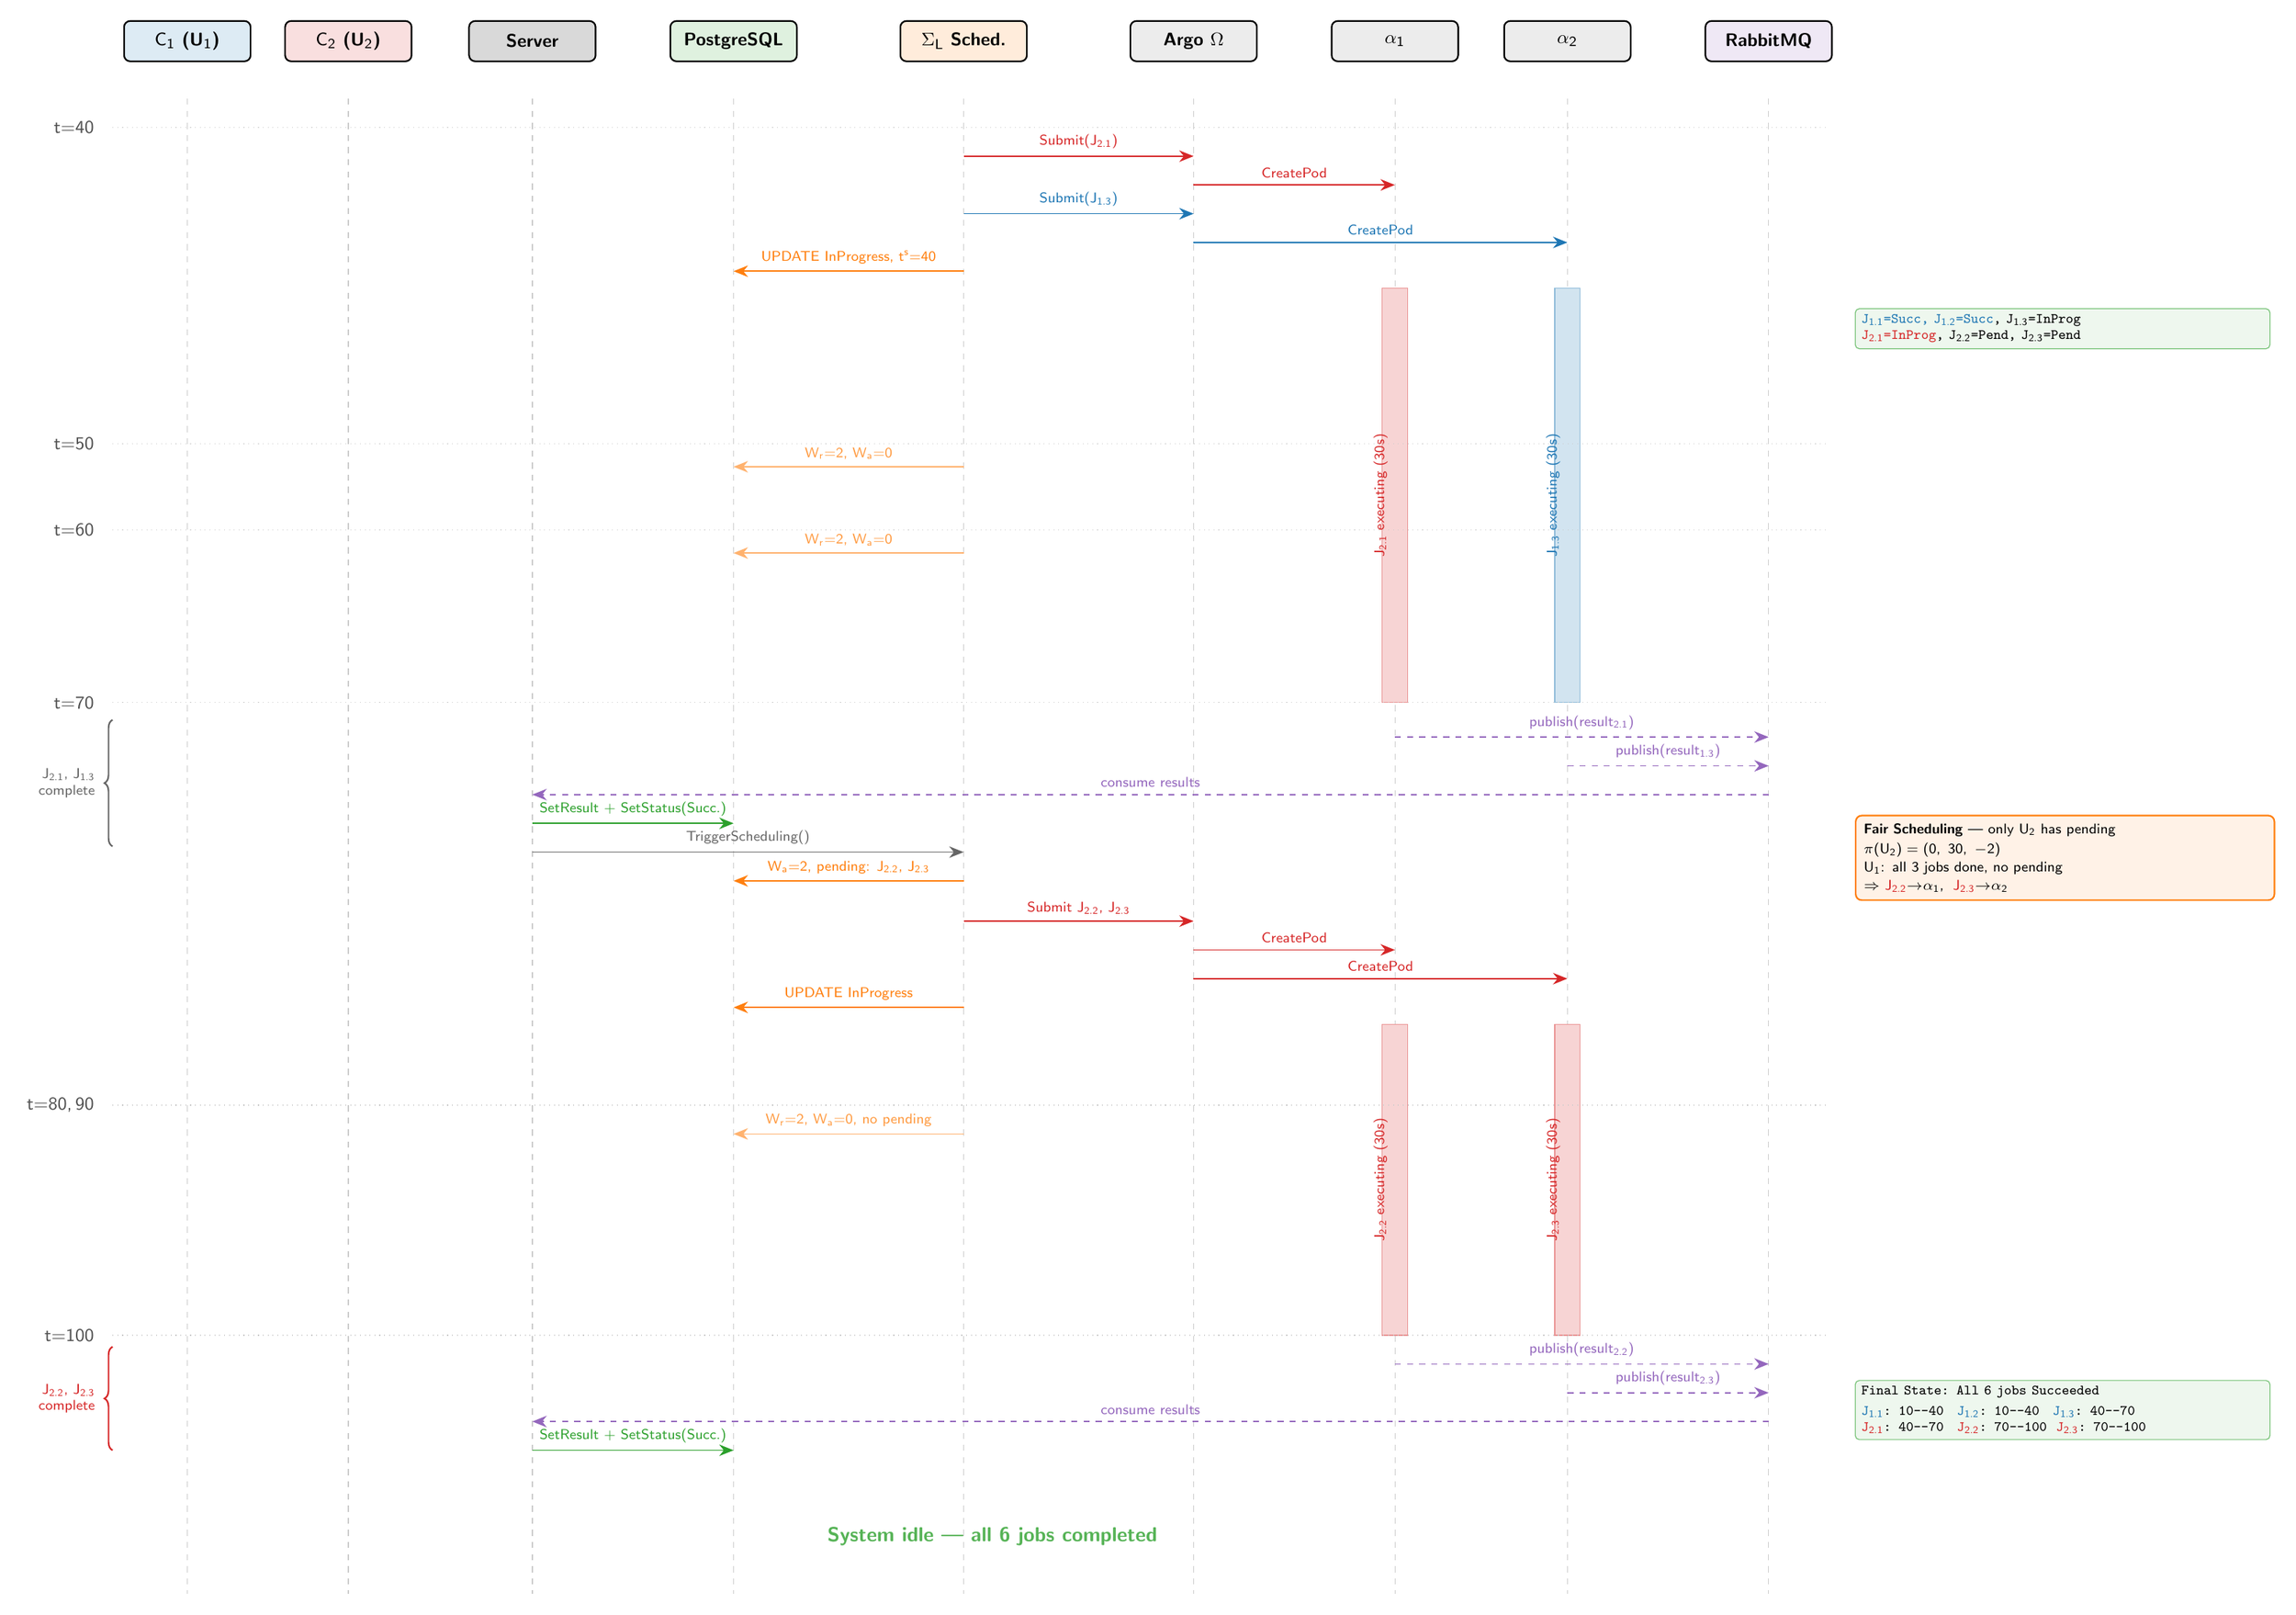
\begin{tikzpicture}[
  x=1cm, y=1cm,
  %
  % Arrow styles
  msg/.style    = {-{Stealth[length=2.5mm, width=2mm]}, semithick, #1},
  msg/.default  = {black},
  amsg/.style   = {-{Stealth[length=2.5mm, width=2mm]}, semithick, dashed, #1},
  amsg/.default = {black},
  %
  % Participant header box
  partbox/.style = {draw, thick, rounded corners=3pt, minimum width=2.2cm,
                    minimum height=0.7cm, font=\small\bfseries, fill=#1!15,
                    text=black},
  %
  % Annotation styles
  note/.style    = {draw, rounded corners=2pt, fill=yellow!12,
                    font=\scriptsize, text width=#1, align=left, inner sep=3pt},
  note/.default  = {3.5cm},
  schedbox/.style = {draw=schedcol, thick, rounded corners=3pt, fill=schedcol!10,
                     font=\scriptsize, text width=#1, align=left, inner sep=4pt},
  schedbox/.default = {5cm},
  dbstate/.style = {draw=dbcol!70, rounded corners=2pt, fill=dbcol!8,
                    font=\scriptsize\ttfamily, text width=#1, align=left, inner sep=3pt},
  dbstate/.default = {5.5cm},
  %
  % Time label
  tmark/.style = {font=\small\bfseries, text=timecol, anchor=east},
]

% Participant x-positions (same as page 1)
\def\xCone{0}
\def\xCtwo{2.8}
\def\xS{6}
\def\xDB{9.5}
\def\xSigma{13.5}
\def\xOmega{17.5}
\def\xAone{21}
\def\xAtwo{24}
\def\xMQ{27.5}
\def\xAnnot{29}
\def\tlx{-1.5}

% Lifeline extent
\def\yTop{-1}
\def\yBot{-27}

% ======================================================================
% PARTICIPANT HEADERS
% ======================================================================
\node[partbox=u1]       at (\xCone,  0) {$C_1$ (U$_1$)};
\node[partbox=u2]       at (\xCtwo,  0) {$C_2$ (U$_2$)};
\node[partbox=black]    at (\xS,     0) {Server};
\node[partbox=dbcol]    at (\xDB,    0) {PostgreSQL};
\node[partbox=schedcol] at (\xSigma, 0) {$\Sigma_L$ Sched.};
\node[partbox=argocol]  at (\xOmega, 0) {Argo $\Omega$};
\node[partbox=argocol]  at (\xAone,  0) {$\alpha_1$};
\node[partbox=argocol]  at (\xAtwo,  0) {$\alpha_2$};
\node[partbox=mqcol]    at (\xMQ,    0) {RabbitMQ};

% ======================================================================
% LIFELINES
% ======================================================================
\foreach \x in {\xCone, \xCtwo, \xS, \xDB, \xSigma, \xOmega, \xAone, \xAtwo, \xMQ} {
  \draw[dashed, gray!40] (\x, \yTop) -- (\x, \yBot);
}

% ======================================================================
% t=40 (cont.): SUBMIT JOBS FROM SCHEDULING DECISION
% ======================================================================
\node[tmark] at (\tlx, -1.5) {$t{=}40$};
\draw[dotted, timecol!30] (-1.3, -1.5) -- (\xMQ+1, -1.5);

% Sigma -> Omega: submit J_2.1
\draw[msg=u2] (\xSigma, -2) -- (\xOmega, -2)
  node[midway, above, font=\scriptsize, text=u2] {Submit(J$_{2.1}$)};

\draw[msg=u2] (\xOmega, -2.5) -- (\xAone, -2.5)
  node[midway, above, font=\scriptsize] {CreatePod};

% Sigma -> Omega: submit J_1.3
\draw[msg=u1] (\xSigma, -3) -- (\xOmega, -3)
  node[midway, above, font=\scriptsize, text=u1] {Submit(J$_{1.3}$)};

\draw[msg=u1] (\xOmega, -3.5) -- (\xAtwo, -3.5)
  node[midway, above, font=\scriptsize] {CreatePod};

% Sigma -> DB: update
\draw[msg=schedcol] (\xSigma, -4) -- (\xDB, -4)
  node[midway, above, font=\scriptsize] {UPDATE InProgress, $t^s{=}40$};

% Activity bars (J_2.1 on alpha_1, J_1.3 on alpha_2)
\fill[u2!20, draw=u2!50] (\xAone-0.22, -4.3) rectangle (\xAone+0.22, -11.5);
\node[font=\scriptsize, text=u2, rotate=90, anchor=south] at (\xAone, -7.9)
  {J$_{2.1}$ executing (30s)};

\fill[u1!20, draw=u1!50] (\xAtwo-0.22, -4.3) rectangle (\xAtwo+0.22, -11.5);
\node[font=\scriptsize, text=u1, rotate=90, anchor=south] at (\xAtwo, -7.9)
  {J$_{1.3}$ executing (30s)};

% DB state at t=40
\node[dbstate=7cm, anchor=west] at (\xAnnot, -5) {%
  \textcolor{u1}{J$_{1.1}$=Succ, J$_{1.2}$=Succ}, J$_{1.3}$=InProg\\
  \textcolor{u2}{J$_{2.1}$=InProg}, J$_{2.2}$=Pend, J$_{2.3}$=Pend
};

% ======================================================================
% t=50, t=60: SCHEDULER POLLS, NO SLOTS
% ======================================================================
\node[tmark] at (\tlx, -7) {$t{=}50$};
\draw[dotted, timecol!30] (-1.3, -7) -- (\xMQ+1, -7);
\draw[msg=schedcol!60] (\xSigma, -7.4) -- (\xDB, -7.4)
  node[midway, above, font=\scriptsize, text=schedcol!80] {$W_r{=}2$, $W_a{=}0$};

\node[tmark] at (\tlx, -8.5) {$t{=}60$};
\draw[dotted, timecol!30] (-1.3, -8.5) -- (\xMQ+1, -8.5);
\draw[msg=schedcol!60] (\xSigma, -8.9) -- (\xDB, -8.9)
  node[midway, above, font=\scriptsize, text=schedcol!80] {$W_r{=}2$, $W_a{=}0$};

% ======================================================================
% t=70: JOBS J_2.1, J_1.3 COMPLETE
% ======================================================================
\node[tmark] at (\tlx, -11.5) {$t{=}70$};
\draw[dotted, timecol!30] (-1.3, -11.5) -- (\xMQ+1, -11.5);

\draw[decorate, decoration={brace, amplitude=4pt, mirror}, thick, black!60]
  (\tlx+0.2, -11.8) -- (\tlx+0.2, -14)
  node[midway, left=5pt, font=\scriptsize, align=right] {J$_{2.1}$, J$_{1.3}$\\complete};

% Results via MQ
\draw[amsg=mqcol] (\xAone, -12.1) -- (\xMQ, -12.1)
  node[midway, above, font=\scriptsize, text=mqcol] {publish(result$_{2.1}$)};

\draw[amsg=mqcol] (\xAtwo, -12.6) -- (\xMQ, -12.6)
  node[midway, above, font=\scriptsize, text=mqcol] {publish(result$_{1.3}$)};

\draw[amsg=mqcol] (\xMQ, -13.1) -- (\xS, -13.1)
  node[midway, above, font=\scriptsize, text=mqcol] {consume results};

\draw[msg=dbcol] (\xS, -13.6) -- (\xDB, -13.6)
  node[midway, above, font=\scriptsize] {SetResult + SetStatus(Succ.)};

\draw[msg=black!60] (\xS, -14.1) -- (\xSigma, -14.1)
  node[midway, above, font=\scriptsize] {TriggerScheduling()};

% Scheduling
\draw[msg=schedcol] (\xSigma, -14.6) -- (\xDB, -14.6)
  node[midway, above, font=\scriptsize] {$W_a{=}2$, pending: J$_{2.2}$, J$_{2.3}$};

\node[schedbox=7cm, anchor=west] at (\xAnnot, -14.2) {%
  \textbf{Fair Scheduling} --- only U$_2$ has pending\\[2pt]
  $\pi(\text{U}_2) = (0,\; 30,\; {-}2)$\\[1pt]
  U$_1$: all 3 jobs done, no pending\\[1pt]
  $\Rightarrow$ \textcolor{u2}{J$_{2.2}$}${\to}\alpha_1$,\;
  \textcolor{u2}{J$_{2.3}$}${\to}\alpha_2$
};

% Submit
\draw[msg=u2] (\xSigma, -15.3) -- (\xOmega, -15.3)
  node[midway, above, font=\scriptsize, text=u2] {Submit J$_{2.2}$, J$_{2.3}$};

\draw[msg=u2] (\xOmega, -15.8) -- (\xAone, -15.8)
  node[midway, above, font=\scriptsize] {CreatePod};
\draw[msg=u2] (\xOmega, -16.3) -- (\xAtwo, -16.3)
  node[midway, above, font=\scriptsize] {CreatePod};

\draw[msg=schedcol] (\xSigma, -16.8) -- (\xDB, -16.8)
  node[midway, above, font=\scriptsize] {UPDATE InProgress};

% Activity bars
\fill[u2!20, draw=u2!50] (\xAone-0.22, -17.1) rectangle (\xAone+0.22, -22.5);
\node[font=\scriptsize, text=u2, rotate=90, anchor=south] at (\xAone, -19.8)
  {J$_{2.2}$ executing (30s)};

\fill[u2!20, draw=u2!50] (\xAtwo-0.22, -17.1) rectangle (\xAtwo+0.22, -22.5);
\node[font=\scriptsize, text=u2, rotate=90, anchor=south] at (\xAtwo, -19.8)
  {J$_{2.3}$ executing (30s)};

% ======================================================================
% t=80, t=90: abbreviated
% ======================================================================
\node[tmark] at (\tlx, -18.5) {$t{=}80,90$};
\draw[dotted, timecol!30] (-1.3, -18.5) -- (\xMQ+1, -18.5);
\draw[msg=schedcol!60] (\xSigma, -19) -- (\xDB, -19)
  node[midway, above, font=\scriptsize, text=schedcol!80] {$W_r{=}2$, $W_a{=}0$, no pending};

% ======================================================================
% t=100: ALL JOBS COMPLETE
% ======================================================================
\node[tmark] at (\tlx, -22.5) {$t{=}100$};
\draw[dotted, timecol!30] (-1.3, -22.5) -- (\xMQ+1, -22.5);

\draw[decorate, decoration={brace, amplitude=4pt, mirror}, thick, u2]
  (\tlx+0.2, -22.7) -- (\tlx+0.2, -24.5)
  node[midway, left=5pt, font=\scriptsize, text=u2, align=right] {J$_{2.2}$, J$_{2.3}$\\complete};

\draw[amsg=mqcol] (\xAone, -23) -- (\xMQ, -23)
  node[midway, above, font=\scriptsize, text=mqcol] {publish(result$_{2.2}$)};
\draw[amsg=mqcol] (\xAtwo, -23.5) -- (\xMQ, -23.5)
  node[midway, above, font=\scriptsize, text=mqcol] {publish(result$_{2.3}$)};

\draw[amsg=mqcol] (\xMQ, -24) -- (\xS, -24)
  node[midway, above, font=\scriptsize, text=mqcol] {consume results};

\draw[msg=dbcol] (\xS, -24.5) -- (\xDB, -24.5)
  node[midway, above, font=\scriptsize] {SetResult + SetStatus(Succ.)};

% Final state
\node[dbstate=7cm, anchor=west] at (\xAnnot, -23.8) {%
  \textbf{Final State:} All 6 jobs Succeeded\\[2pt]
  \textcolor{u1}{J$_{1.1}$}: 10--40\;\;
  \textcolor{u1}{J$_{1.2}$}: 10--40\;\;
  \textcolor{u1}{J$_{1.3}$}: 40--70\\
  \textcolor{u2}{J$_{2.1}$}: 40--70\;\;
  \textcolor{u2}{J$_{2.2}$}: 70--100\;
  \textcolor{u2}{J$_{2.3}$}: 70--100
};

\node[font=\normalsize\bfseries, text=dbcol!80] at (14, -26) {System idle --- all 6 jobs completed};

\end{tikzpicture}%
}% end makebox

\end{document}

%%% Local Variables:
%%% mode: LaTeX
%%% TeX-master: t
%%% TeX-engine: luatex
%%% TeX-command-extra-options: "-synctex=1 -shell-escape -interaction=nonstopmode"
%%% End:
